\section{In-context learning}

A surprising property of large language models is their emergent ability to learn \textit{in-context}, that is, their ability to learn a task without updating any parameters at all. The name `in-context' comes from the fact that the learning is done by simply including several examples or a task description (or both!) prepended to a test input present to the model

For example, for a question-answering task, to make a 2-shot prediction for a test input `Why is the sky blue?', rather than presenting the input:

\texttt{Why is the sky blue?\textless generate\textgreater}

we would simply prepend our 2 examples to the input:

\texttt{Who is the US president? Joe Biden What is earth's tallest mountain? Mount... \\
Everest Why is the sky blue?\textless generate\textgreater}

In addition to few-shot in-context learning, models can often improve their zero-shot generalization if the input is formatted in a particular manner; for example, adding a \texttt{Q:} and \texttt{A:} prefix to the input and label, respectively:

\texttt{Q: Why is the sky blue? A:\textless generate\textgreater}

Finally, these two approaches can be combined, for example adding the \texttt{Q:} and \texttt{A:} markers to each example in the context as well as the test input.

\begin{enumerate}[label={2.\alph*}]
    \item \points{2a} {\bf Implement In-Context Learning}

Complete the code for in-context learning in \texttt{icl.py}.
\begin{enumerate}[label=(\roman*)]
    \item Implement prompt creation for the XSum and bAbI tasks, which is found in \texttt{icl.py:get\_icl\_prompts()}. You will implement 4 prompt format modes:
    \begin{enumerate}[label={\arabic*}]
        \item \texttt{qa} \textbf{[only for bAbI]}: Add ``\texttt{ In the }'' after the question (including the final test question that we want to generate an answer for!) and before each answer, since this task involves answering questions about the physical whereabouts of a person. In addition, add a period after the answer (omitting the period can significantly impact your results!). Be sure to include a space between the question and \texttt{In the}, as well as a space before the answer (though keep in mind Note 1!). Note the  \texttt{Q:} and \texttt{A:} prompts in the example earlier don't apply here.
        \item \texttt{none} \textbf{[only for XSum]}: In this case, we use the raw $k$ examples without any additional formatting; that is, we just concatenate $[x_1; y_1; ... ; \allowbreak x_k; y_k; x^*]$ with a space between each element (but no space at the end), where $x^*$ is the input that we want to generate an answer for.
        \item \texttt{tldr} \textbf{[only for XSum]}: Add the text ``\texttt{ TL;DR: }'' after each article/input (including the final test article) and before the summary/target.
        \item \texttt{custom} \textbf{[only for XSum]}: Come up with your own prompt format for article summarization (different from the ones we've shown!).
    \end{enumerate}
    In general, the idea of in-context learning is to format the support examples in the same way as the test example, to leverage the model's tendency toward imitation.

    \textbf{Note 1: Due to a quirk with GPT-2 tokenization, you should not include a space at the end of your prompt before generation.}
    
    \textbf{Note 2: Be sure to shuffle the order of the support inputs/targets when you construct the prompt (we will need this randomization later).}
    \item Implement greedy sampling in \texttt{icl.py:do\_sample()}. The GPT-2 models used in this and the following questions use an autoregressive factorization of the probability of a sequence, i.e. $p_\theta(\mathbf{x}) = \prod_t p_\theta(x_t \mid x_{<t})$. `Greedy' sampling means that given a context $x_{<t}$ producing a distribution over next tokens $p_\theta(x_t \mid x_{<t})$, we deterministically choose the next token $x_t$ to be the token with highest probability.
    
    \textbf{Note 3: Be sure you understand what each dimension of the model's output \texttt{logits} represents. Misinterpreting the dimensions of this output can lead to subtle bugs.}
    
    \item Finally, put the pieces together by completing the implementation of \texttt{icl.py:\allowbreak run\_icl()}, using your \texttt{get\_icl\_prompts()} and \texttt{do\_sample()} functions, as well as the HuggingFace tokenizer defined in the loop. \\ \emph{Hint}: Your solution here should be less than 5 lines of code.
\end{enumerate}
    \item {\bf Evaluate on bAbI}

\begin{enumerate}[label=(\roman*)]
    \item \points{2bi} {\bf Run ICL on bAbI}

First, evaluate $k$-shot in-context performance on bAbI for GPT-2-medium (355M parameters) and full-size GPT-2 (1.5B parameters) for various values of $k$ with the command:
    
\texttt{\small python3 main.py --task run\_icl --model med,full --dataset babi --k 0,1,16}

Plot the results with the command:

\texttt{\small python3 main.py --task plot\_icl --model med,full --dataset babi --k 0,1,16}

Your plots should look like:
\begin{center}
    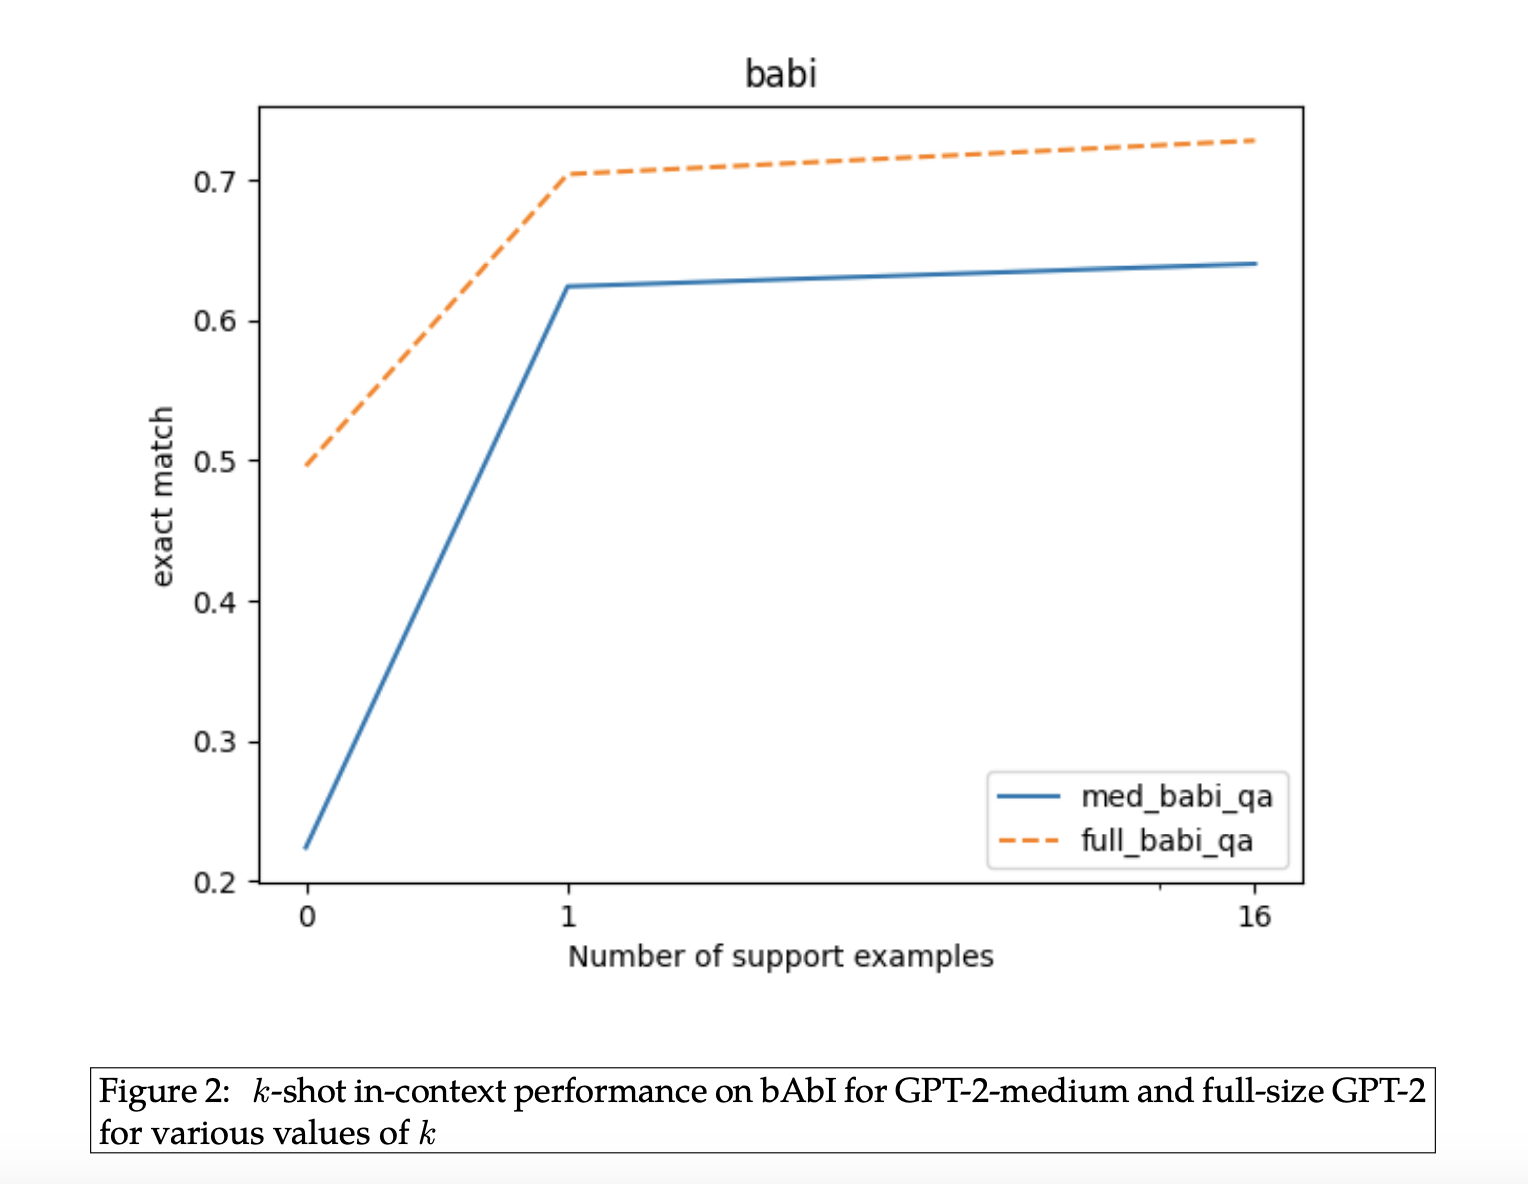
\includegraphics[width=0.75\linewidth]{./figures/incontext-2b}
\end{center}

    \item \points{2bii} {\bf Reason on ICL on bAbI}


What relationship(s) do you notice between model scale and few-shot performance?
\end{enumerate}

    \item {\bf Evaluate on XSum}

\begin{enumerate}[label=(\roman*)]
    \item \points{2ci} {\bf Run ICL on XSum}

Now let's evaluate several different prompt formats on the XSum dataset. With and without a task description in the prompt, evaluate zero-shot and few-shot performance for XSum on GPT-2-Medium with the command:

\texttt{\small python3 main.py --task run\_icl --model med,full --dataset xsum --k 0,1,4 \textbackslash \\
\phantom{asdf}--prompt none,tldr,custom}

Note that we use much smaller $k$ than in the previous problem, because we must fit all $k$ examples into the model's context window, which is only 1024 tokens. The fixed context window length is one limitation of in-context learning.

\textbf{The $k=4$ XSum evaluation on full-size GPT-2 may take approximately 40 minutes on your Azure instance for each prompt mode}; this is expected, and is another downside of in-context learning (we need to process a much longer input, containing the prompt, compared to a fine-tuned model that just processes the test input).

Plot the zero-shot and few-shot performance of GPT-2 on XSum:

\texttt{\small python3 main.py --task plot\_icl --model med,full --dataset xsum --k 0,1,4 \textbackslash \\
\phantom{asdf}--prompt none,tldr,custom}

Your plot should look like:
\begin{center}
    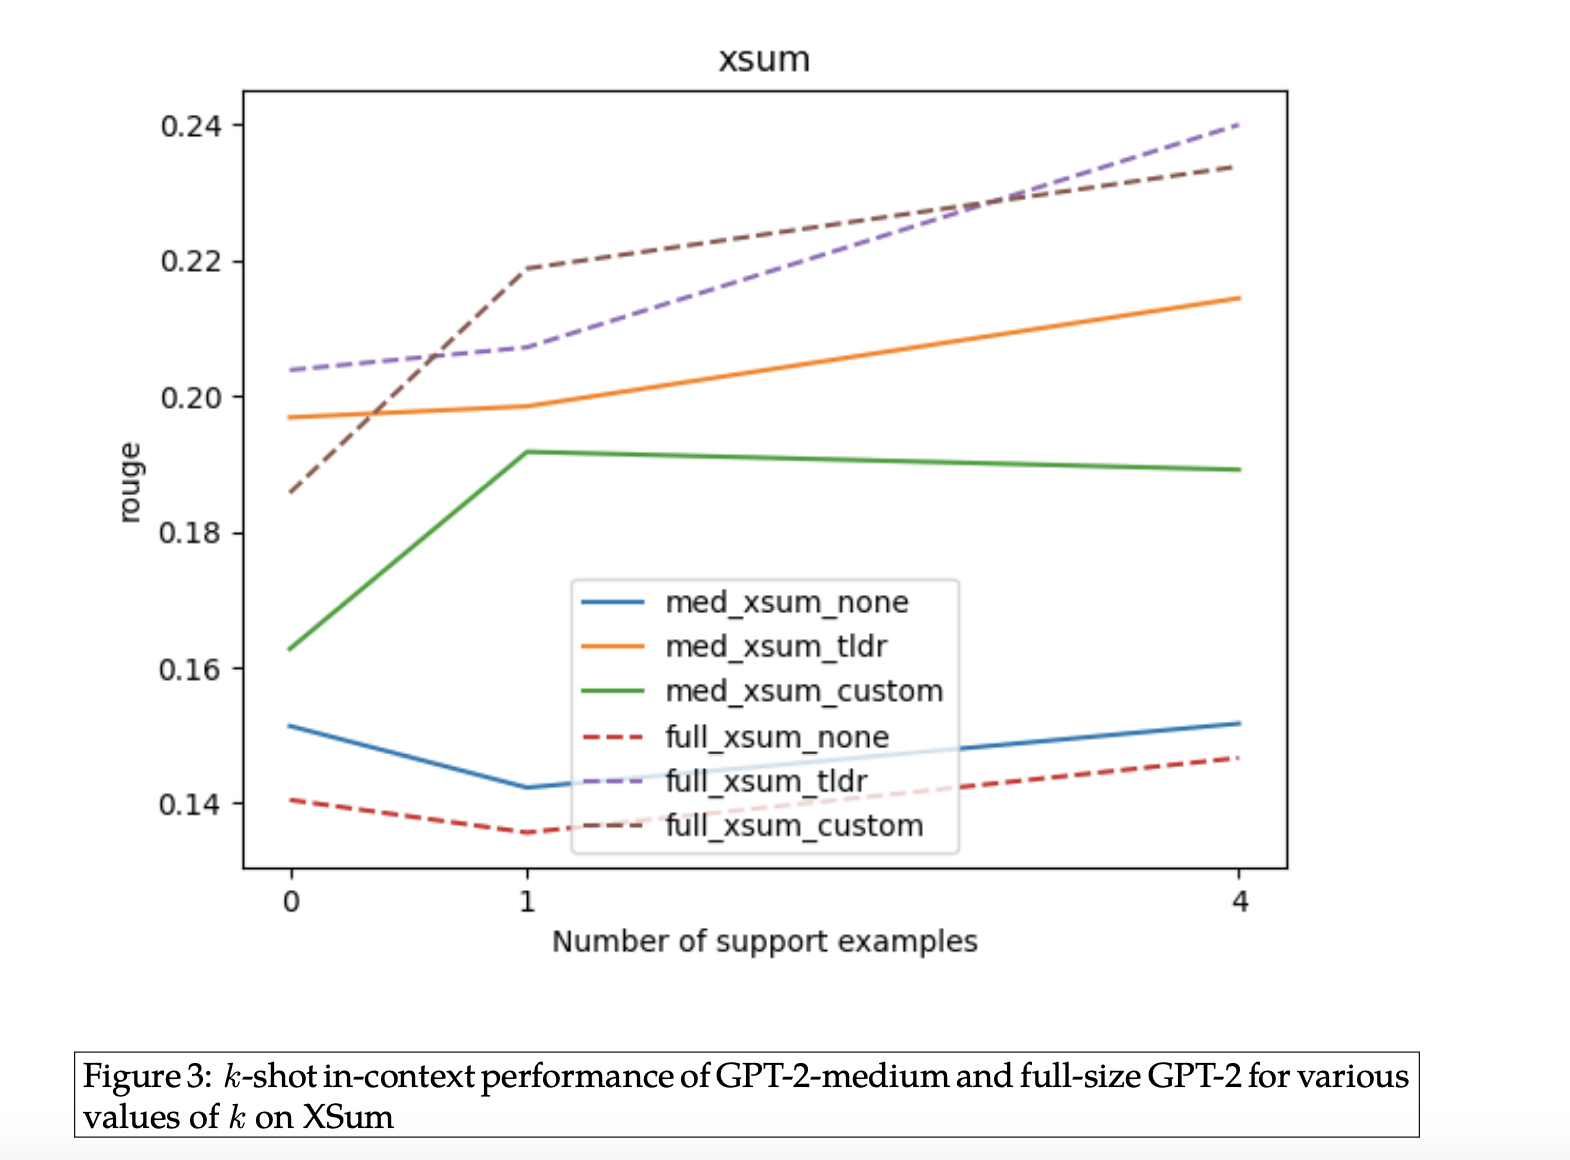
\includegraphics[width=0.75\linewidth]{./figures/incontext-2c}
\end{center}


    \item \points{2cii} {\bf Reason on ICL on XSum}

How does the performance of the \texttt{TL;DR:} prompt compare with no prompt formatting? What was your custom prompt format, and how did it compare with \texttt{TL;DR:}? Discuss the relative performance of the different prompts in the zero-shot, one-shot, and few-shot settings.

\end{enumerate}

\end{enumerate}